\documentclass[titlepage]{article}
\usepackage{amsfonts}
\usepackage{bbm}
\usepackage{graphicx}
\renewcommand{\baselinestretch}{1}
\usepackage[utf8]{inputenc}
\usepackage{color}
\usepackage[T1]{fontenc}
\usepackage{geometry}
\usepackage{amsmath}
\usepackage{enumerate}
\usepackage{caption}
\usepackage{graphicx}
\usepackage{subcaption}
\usepackage{array}
\usepackage{fullpage}
\usepackage{algorithm2e}
\usepackage{float}
\usepackage{listings}
\usepackage{tikz}
\everymath{\displaystyle}

\newtheorem{theorem}{Theorem}[section]
\newtheorem{lemma}[theorem]{Lemma}
\newtheorem{proposition}[theorem]{Proposition}
\newtheorem{corollary}[theorem]{Corollary}

\newenvironment{proof}[1][Proof]{\begin{trivlist}
\item[\hskip \labelsep {\bfseries #1}]}{\end{trivlist}}
\newenvironment{definition}[1][Definition]{\begin{trivlist}
\item[\hskip \labelsep {\bfseries #1}]}{\end{trivlist}}
\newenvironment{example}[1][Example]{\begin{trivlist}
\item[\hskip \labelsep {\bfseries #1}]}{\end{trivlist}}
\newenvironment{remark}[1][Remark]{\begin{trivlist}
\item[\hskip \labelsep {\bfseries #1}]}{\end{trivlist}}

\newcommand{\qed}{\nobreak \ifvmode \relax \else
      \ifdim\lastskip<1.5em \hskip-\lastskip
      \hskip1.5em plus0em minus0.5em \fi \nobreak
      \vrule height0.75em width0.5em depth0.25em\fi}


\begin{document}
\title{Coach Ranking Model}
\author{Akilesh Potti, Dominick Twitty, Wenhai Yang}
\maketitle

\begin{abstract}
Todo
\end{abstract}



\noindent\textbf{Disclaimer:} For legal and moral reasons, all geographical locations and company names used in this paper are entirely fictional unless otherwise stated. However, for the sake of accuracy, real world data was used to tune our model.


\section{The Problem}
\begin{enumerate}
\item Todo
\end{enumerate}


\section{Model assumptions}
\begin{enumerate}
\item Todo
\end{enumerate}

\section{Models}

\subsection{Simple Heuristic Model}
\subsubsection{Sorting by Win/Loss Ratio}
\subsubsection{Sorting by Net Wins}
\subsubsection{Differentiate between Games}



\subsection{Machine Learning Model}



\subsection{Graphical Model}
It comes very natural for us to consider the problem as a graph. The nodes of the graph are the coaches. An edge between two nodes denotes the relation between two coaches, such as the game result of them playing against each other.
\\

\noindent This idea of representing the problem as a graph is a very good step forward because it allow us to go beyond the simple statistics like win/loss ratio of a single coach, and gain more insight from the data.
\\

\noindent Another advantage of this model is that it can aggregate data from different time periods. For example if coach A beats coach B and then retired in 1990, and coach B beat coach C later in 1995, then in the graph we will have a way to compare coach A and coach C because there is a path from A to C through B, even though they never played against each other.

\subsubsection{Topolical Ordering}
A very first idea that comes to mind is Topological Ordering. In this sub-model, there exist an edge from $i$ to $j$ if and only if among all the games $i$ played against $j$, $i$ beat $j$ more often than $j$ beat $i$. Then if there exists a Topological Ordering of the graph, we have a ranking of the coaches based on their rival history.
\\

\noindent Consider the following example. Coach 1 has been beaten by both 2 and 3, coach 2 has been beaten by coach 3 and 4, coach 3 has been beaten by coach 4, and coach 4 is never beaten by anyone. We have a topological ordering in the graph: $\{1, 2, 3, 4\}$, and it is natural to conclude that coach 4 is the best coach among them.

\begin{center}
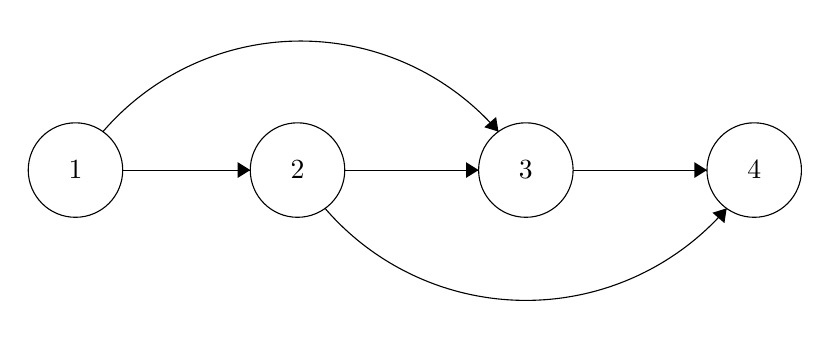
\begin{tikzpicture}[scale=0.2]
\tikzstyle{every node}+=[inner sep=0pt]
\draw [black] (16.1,-27.9) circle (3);
\draw (16.1,-27.9) node {$1$};
\draw [black] (30.2,-27.9) circle (3);
\draw (30.2,-27.9) node {$2$};
\draw [black] (44.7,-27.9) circle (3);
\draw (44.7,-27.9) node {$3$};
\draw [black] (59.2,-27.9) circle (3);
\draw (59.2,-27.9) node {$4$};
\draw [black] (19.1,-27.9) -- (27.2,-27.9);
\fill [black] (27.2,-27.9) -- (26.4,-27.4) -- (26.4,-28.4);
\draw [black] (33.2,-27.9) -- (41.7,-27.9);
\fill [black] (41.7,-27.9) -- (40.9,-27.4) -- (40.9,-28.4);
\draw [black] (47.7,-27.9) -- (56.2,-27.9);
\fill [black] (56.2,-27.9) -- (55.4,-27.4) -- (55.4,-28.4);
\draw [black] (17.843,-25.463) arc (139.24738:40.75262:16.577);
\fill [black] (42.96,-25.46) -- (42.81,-24.53) -- (42.06,-25.18);
\draw [black] (57.453,-30.334) arc (-40.77401:-139.22599:16.84);
\fill [black] (57.45,-30.33) -- (56.55,-30.61) -- (57.31,-31.27);
\end{tikzpicture}
\end{center}

\noindent However, one natural limitation of this model is the following theorem:

\begin{theorem}
A graph $G$ has a topological ordering if and only if it is a DAG (directed acyclic graph).
\end{theorem}
\begin{proof}
See Section 3.6 of Algorithms Design by Kleinberg and Tardos.
\end{proof}

\noindent To solve this issue, we think of an algorithm to reduce the originial graph into a DAG: keep removing the most "unimportant" untils the graph is acyclic. By most "unimportant" we then have to find a way to measure the significance of superiority of one coach against another.
\\

\begin{algorithm}[H]
\caption{Graph Reduction Algorithm}
\end{algorithm}
\begin{algorithm}[H]


\While{$G$ is not a DAG}{
$e$ = edge with the least importance in $G$\;
Remove $e$ from $G$
}

\end{algorithm}



\subsubsection{Markov Chain}

\begin{center}
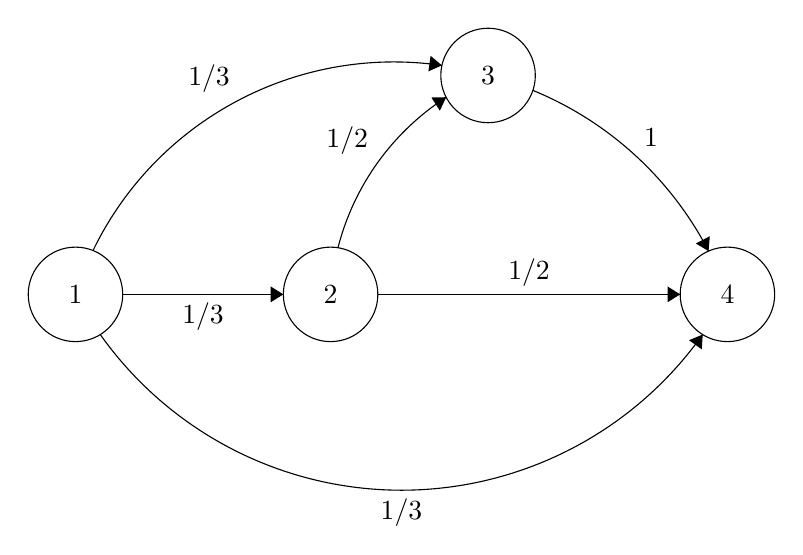
\begin{tikzpicture}[scale=0.2]
\tikzstyle{every node}+=[inner sep=0pt]
\draw [black] (14.8,-32.3) circle (3);
\draw (14.8,-32.3) node {$1$};
\draw [black] (31,-32.3) circle (3);
\draw (31,-32.3) node {$2$};
\draw [black] (41,-18.4) circle (3);
\draw (41,-18.4) node {$3$};
\draw [black] (56.2,-32.3) circle (3);
\draw (56.2,-32.3) node {$4$};
\draw [black] (15.913,-29.517) arc (154.15261:81.74236:21.233);
\fill [black] (38.07,-17.76) -- (37.35,-17.15) -- (37.21,-18.14);
\draw (23.28,-19.51) node [above] {$1/3$};
\draw [black] (17.8,-32.3) -- (28,-32.3);
\fill [black] (28,-32.3) -- (27.2,-31.8) -- (27.2,-32.8);
\draw (22.9,-32.8) node [below] {$1/3$};
\draw [black] (54.626,-34.851) arc (-35.33903:-144.66097:23.446);
\fill [black] (54.63,-34.85) -- (53.76,-35.21) -- (54.57,-35.79);
\draw (35.5,-45.24) node [below] {$1/3$};
\draw [black] (34,-32.3) -- (53.2,-32.3);
\fill [black] (53.2,-32.3) -- (52.4,-31.8) -- (52.4,-32.8);
\draw (43.6,-31.8) node [above] {$1/2$};
\draw [black] (31.468,-29.341) arc (165.67502:122.86066:16.127);
\fill [black] (38.34,-19.78) -- (37.4,-19.8) -- (37.94,-20.64);
\draw (33.41,-22.54) node [left] {$1/2$};
\draw [black] (43.845,-19.346) arc (67.6945:27.42131:21.964);
\fill [black] (55,-29.55) -- (55.08,-28.61) -- (54.19,-29.07);
\draw (51.35,-22.97) node [above] {$1$};
\end{tikzpicture}
\end{center}



\section{Results, Validation, and Robustness}

\begin{figure}[H]
      \centering
      \begin{subfigure}{0.48\textwidth}
	\caption{Distribution of Request Source with Airport}
      \centering
      \includegraphics[width=1.1\textwidth]{src_with_airport.jpg}
      \end{subfigure}\quad
      \begin{subfigure}{0.48\textwidth}
	\caption{Distribution of Request Source without Airport}
      \centering
      \includegraphics[width=1.1\textwidth]{src_without_airport.jpg}
      \end{subfigure}
      \begin{subfigure}{0.48\textwidth}
	\caption{Distribution of Request Destination with Airport}
      \centering
      \includegraphics[width=1.1\textwidth]{dest_with_airport.jpg}
      \end{subfigure}\quad
      \begin{subfigure}{0.48\textwidth}
	\caption{Distribution of Request Destination without Airport}
      \centering
      \includegraphics[width=1.1\textwidth]{dest_without_airport.jpg}
      \end{subfigure}
 \end{figure}

$$p_{unreg} = k \ln (t_{reg})$$
$$\frac{p_{unreg'}}{p_{unreg}}  = \frac{\ln_{t_{reg}}}{ \ln{t_{reg'}}}$$

\begin{center}
\begin{tabular}{ | c | c | c | c | c | c | c | c | c | }
\hline
 Number of Cabs & 14 & 15 & 16 & 17 & 18 & 19 & 20 & 21 \\\hline
Uni Ind/Conglo & 1.5720  &  1.3773  &  1.2880 &   1.2071 &   1.1932 &  1.2113  &  1.1201  &  1.0672\\\hline
Prop Ind/Conglo & 1.6876  &  1.4040  &  1.2459  &  1.1248  &  1.2558  &  1.1498  &  1.1033  &  1.1022\\\hline
Disprop Ind/Conglo & 2.1519  &  2.0706 &   2.0489  &  1.9399  &  1.8725 &   1.8174  &  1.6990 &   1.3905\\
\hline
\end{tabular}
\end{center}

\section{Strengths and Weaknesses}
\subsection{Strengths}
\begin{itemize}
\item Todo
\end{itemize}
\subsection{Weaknesses}
\begin{itemize}
\item Todo
\end{itemize}

\section{Conclusions}
Todo

\section{Future work}
\begin{itemize}
\item Todo
\end{itemize}

\pagebreak

\section{Bibliography}
\begin{thebibliography}{9}

\bibitem{OSM} OpenStreetMaps API,
\verb|http://www.openstreetmap.org/#map=14/42.4427/-76.4984|
\bibitem{Gist} Github Gist by user aflaxman,
\verb|https://gist.github.com/aflaxman/287370/|
\bibitem{Re} $\text{A stochastic optimization model for real-time ambulance redeployment}$,
\\\verb|http://www.sciencedirect.com/science/article/pii/S0305054813000385|
\bibitem{Ithaca} Ithaca Demographics,
\verb|http://www.ci.ithaca.ny.us/maps/index.cfm|
\bibitem{Cornell} Cornell Demographics,
\verb|http://www.cornell.edu/about/facts/stats.cfm|
\bibitem{IC} Ithaca College,
\verb|http://www.ithaca.edu/admission/facts/|


\end{thebibliography}

\pagebreak

\section{Code}


\definecolor{mygreen}{rgb}{0,0.6,0}
\definecolor{mygray}{rgb}{0.5,0.5,0.5}
\definecolor{mymauve}{rgb}{0.58,0,0.82}

\lstset{ %	
  backgroundcolor=\color{white},   % choose the background color; you must add \usepackage{color} or \usepackage{xcolor}
  basicstyle=\footnotesize,        % the size of the fonts that are used for the code
  breakatwhitespace=false,         % sets if automatic breaks should only happen at whitespace
  breaklines=true,                 % sets automatic line breaking
  captionpos=b,                    % sets the caption-position to bottom
  commentstyle=\color{mygreen},    % comment style
  deletekeywords={...},            % if you want to delete keywords from the given language
  escapeinside={\%*}{*)},          % if you want to add LaTeX within your code
  extendedchars=true,              % lets you use non-ASCII characters; for 8-bits encodings only, does not work with UTF-8
  frame=single,                    % adds a frame around the code
  keepspaces=true,                 % keeps spaces in text, useful for keeping indentation of code (possibly needs columns=flexible)
  keywordstyle=\color{blue},       % keyword style
  morekeywords={*,...},            % if you want to add more keywords to the set
  numbers=left,                    % where to put the line-numbers; possible values are (none, left, right)
  numbersep=5pt,                   % how far the line-numbers are from the code
  numberstyle=\tiny\color{mygray}, % the style that is used for the line-numbers
  rulecolor=\color{black},         % if not set, the frame-color may be changed on line-breaks within not-black text (e.g. comments (green here))
  showspaces=false,                % show spaces everywhere adding particular underscores; it overrides 'showstringspaces'
  showstringspaces=false,          % underline spaces within strings only
  showtabs=false,                  % show tabs within strings adding particular underscores
  stepnumber=2,                    % the step between two line-numbers. If it's 1, each line will be numbered
  stringstyle=\color{mymauve},     % string literal style
  tabsize=2,                       % sets default tabsize to 2 spaces
  title=\lstname,                  % show the filename of files included
  columns=fullflexible,basicstyle=\ttfamily,  
  language=Python    
}
\begin{lstlisting}[frame=none]
\end{lstlisting}

\end{document}